\chapter{Reinforcement Learning}

In this section, we introduce deep reinforcement learning (RL) instead of the classical one, for which one may refer to \emph{Reinforcement Learning: An Introduction} by Sutton.

As for deep RL, \emph{Tutorial on Deep Reinforcement Learning, decision making, and control} in International Conference on Machine Learning(ICML) 2017 is a nice reference.

\section{The Framework of Reinforcement Learning}

We introduce the basic framework of RL with the descriptions in TRPO. This is a general framework adopted in reinforcement learning, which formulates the conception that an agent interacts with the environment, and learns how to get more rewards by modifying its policy.

Consider an infinite-horizon discounted Markov decision process(MDP): 
\begin{itemize}
    \item  $\mathcal{S}$ is a finite set of states, $s\in\mathcal{S}$
    \item $ \mathcal{A}$ is a finite set of actions, $a\in\mathcal{A}$
    \item $\mathcal{P}$ is the transition probability distribution, $\mathcal{P}_{ss'}^{a}:=P(s'|s,a)$
    \item $r$ is a one step reward function, $r(s,a,s')$,or $r(s)$ 
    \item $\gamma\in[0,1]$ is a discount factor
\end{itemize}

The agent can then interact with the environment. At time step $t$, it receives an observation $s_t$(it should be $o_t$, whereas $s_t$ is the true state, but here we identify them for simplicity), and adopts an action $a_t$ from the policy $\pi$, then the environment replies a new state $s_{t+1}$ and a reward $r_t$.

\begin{center}
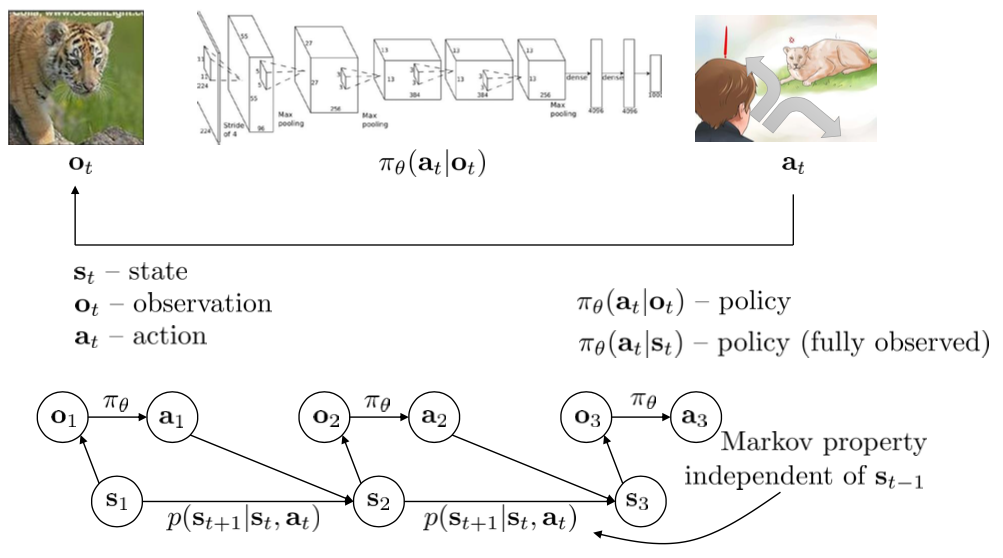
\includegraphics[width=\textwidth]{RLEnv}
\end{center}

As a result, the agent generates a \emph{path} $p=(s_0,a_0,r_0,s_1,\cdots)$.

Based on these notions, we mainly consider the following special functions.
\begin{enumerate}
\item
The expected discounted reward $\eta(\pi)=\mathbb{E}_{s_0, a_0, \cdots}\left[\sum_{t=0}^\infty \gamma^l r(s_t)\right]$
\item
The state-action value function $Q(s_t,a_t)=\mathbb{E}_{s_{1+t},a_{t+1},\cdots}[\sum_{l=0}^\infty\gamma^lr(s_{t+l})]$, which represents the value of the state-action pair $(s,a)$.
\item
The value function $V_{\pi}(s_t)=\mathbb{E}_{a_t,s_{t+1},a_{t+1},\cdots}[\sum_{l=0}^\infty\gamma^lr(s_{t+l})]$, which represents the value of the state $s$.
\item
The advance function $A_\pi(s,a)=Q_{\pi}(s,a)-V_\pi(s)$, which represents the advantage of the action $a$ against the mean value.
\end{enumerate}

One important connection between two distinct policies $\pi$, $\tilde\pi$ is
$$\eta(\tilde\pi)=\eta(\pi)+\mathbb{E}_{s_0,a_0,\cdots|\tilde\pi}[\sum_{t=0}^\infty\gamma^tA_\pi(s_t,a_t)].$$

It has a corollary,
$$ \eta(\tilde\pi)=\eta(\pi)+\sum_s\rho_{\tilde\pi(s)}\sum_a\tilde\pi(a|s)A_{\pi}(s,a)
$$
where
$$ \rho_\pi(s)=P(s_0=s)+\gamma P(s_1=s)+\gamma^2P(s_2=s)+\cdots.
$$
To get this equation, one only need to transform from the last term. We will show the proof later.

Finally, our aim is to find a stochastic policy $\pi(a|s)$ that maximizes the expected discounted reward 
\begin{align*}
\max_{\pi}\eta(\pi)=\mathbb{E}_{\pi}(\sum_{t=0}^{\infty}\gamma^{t}r(s_{t}))
\end{align*}
where $s_{0}\sim P_{0}$, $a_{t}\sim \pi(\cdot|s_{t})$, and $s_{t+1}\sim P(\cdot|s_{t},a_{t})$.

\section{The Vanilla Policy Gradient Method}
We  now briefly summarize a classical training algorithm, also known as the \emph{vanilla}(means \emph{plain}) policy gradient(VPG) method.

Suppose the policy $\pi$ is parametrized by $\theta$, denoted as $\eta=\eta_{\theta}$, and the time is limited by $T$. With the likelihood ratio trick, the gradient of $\eta_{\theta}$ can be written as
\[\nabla_{\theta}\eta(\theta)=\mathbb{E}\left[ \left(\sum_{t=0}^T \gamma^tr(s_t,a_t)\right)\left(\sum_{t=0}^T \nabla_{\theta}\log\pi_{\theta}(a_t|s_t)\right)  \right].\]

Notice that for $t'<t$, we have
\begin{align*}
	&\mathbb{E}[r(s_{t'},a_{t'})\nabla_{\theta}\log\pi_{\theta}(a_t|s_t))]\\
	=&\nabla_{\theta}\mathbb{E}[r(s_{t'},a_{t'})\log\pi_{\theta}(a_t|s_t))]\\
	=&\nabla_{\theta}\mathbb{E}[r(s_{t'},a_{t'})]\\
	=&0.
\end{align*}
We can then reduce the gradient to
\[\nabla_{\theta}\eta(\theta)=\mathbb{E}\left[ \left(\sum_{t'=t}^T \gamma^{t'}r(s_{t'},a_{t'})\right)\left(\sum_{t=0}^T \nabla_{\theta}\log\pi_{\theta}(a_t|s_t)\right)  \right].\]
In practical, we often cut off the extra $\gamma$ in the above formula, and get
\[\nabla_{\theta}\eta(\theta)=\mathbb{E}\left[ \left(\sum_{t'=t}^T \gamma^{t'-t}r(s_{t'},a_{t'})\right)\left(\sum_{t=0}^T \nabla_{\theta}\log\pi_{\theta}(a_t|s_t)\right)  \right].\]
Based on this formula, the empirical policy gradient can be written as
\[\widehat{\nabla_{\theta}\eta_{\theta}}=\frac{1}{NT}\sum_{i=1}^N\sum_{t=0}^{T-1}\nabla_{\theta}\log\pi_{\theta}(a_t|s_t)R_t^i\]
where
\[R_t=\sum_{t'=t}^T\gamma^{t'-t}r(s_{t'},a_{t'}).\]
One can see that VPG is a classical gradient descent(or ascent) method. We need choose a step size $\alpha$ and then update $\theta$ by
\[\theta_{i+1}=\theta_{i}+\alpha\widehat{\nabla_{\theta}\eta_{\theta}}.\]
A lack of VPG is that it gives no guidance to choose $\alpha$. Some algorithms are proposed to solve this problem, among which is TRPO.

\section{The Formulation of TRPO}
Notice that
\begin{align*}
&\mathbb{E}_{\pi}[r(s_{t})+\gamma V_{\pi}(s_{t+1})-V_{\pi}(s_{t})]\\
&=\mathbb{E}_{\pi}[r(s_{t})+\gamma V_{\pi}(s_{t+1})]-V_{\pi}(s_{t})\\
 &=Q_{\pi}(s_{t},a_{t})-V_{\pi}(s_{t})=A_{\pi}(s_{t},a_{t}).
\end{align*}
For two different policies $\tilde{\pi}$ and $\pi$, we have:
\begin{align*}
\mathbb{E}_{\tilde{\pi}}[\sum_{t=0}^{\infty}\gamma^{t}A_{\pi}(s_{t},a_{t})]&=\mathbb{E}_{\tilde{\pi}}[\sum_{t=0}^{\infty}\gamma^{t}\mathbb{E}_{\pi}(r(s_{t})+\gamma V_{\pi}(s_{t+1})-V_{\pi}(s_{t}))]\\
&=\mathbb{E}_{\tilde{\pi}}[\sum_{t=0}^{\infty}\gamma^{t}r(s_{t})+\sum_{t=0}^{\infty}\gamma^{t}\mathbb{E}_{\pi}(\gamma V_{\pi}(s_{t+1})-V_{\pi}(s_{t}))]\\
&=\mathbb{E}_{\tilde{\pi}}(\sum_{t=0}^{\infty}\gamma^{t}r(s_{t}))+\mathbb{E}_{\tilde{\pi}}[\sum_{t=0}^{\infty}\gamma^{t}\mathbb{E}_{\pi}[\gamma V_{\pi}(s_{t+1})-V_{\pi}(s_{t})]]\\
&=\mathbb{E}_{\tilde{\pi}}[\mathbb{E}_{\pi}(-V_{\pi}(s_{0}))]+\eta(\tilde{\pi})=\eta(\tilde{\pi})-\eta(\pi).
\end{align*}
We have omitted the term $\gamma^{t}V_{\pi}(s_{t})\rightarrow0(t\rightarrow\infty)$ in the last equality, since $\gamma^{t}\rightarrow 0(t\rightarrow\infty)$.

Rearrange the terms, we have
\begin{align*}
\eta(\tilde{\pi})&=\eta(\pi)+\mathbb{E}_{\tilde{\pi}}(\sum_{t=0}^{\infty}\gamma^{t}A_{\pi}(s_{t},a_{t}))\\
&=\eta(\pi)+\sum_{t=0}^{\infty}\sum_{s}P(s_{t}=s|\tilde{\pi})\sum_{a}\tilde{\pi}(a|s)\gamma^{t}A_{\pi}(s,a)\\
&=\eta(\pi)+\sum_{s}\sum_{t=0}^{\infty}\gamma^{t}P(s_{t}=s|\tilde{\pi})\sum_{a}\tilde{\pi}(a|s)A_{\pi}(s,a)\\
&=\eta(\pi)+\sum_{s}\rho_{\tilde{\pi}}(s)\sum_{a}\tilde{\pi}(a|s)A_{\pi}(s,a)
\end{align*}

\section{Establishing the Approximater}
To derive a practical algorithm, we consider parameterize the policy as $\pi_{\theta}$. 

Let us propose a local approximation to $\eta(\pi_{\theta})$:
\begin{align}
L_{\pi_{\theta_{old}}}(\pi_{\theta})=\eta(\pi_{\theta_{old}})+\sum_{s}\rho_{\pi_{\theta_{old}}}(s)\sum_{a}\pi_{\theta}(a|s)A_{\pi_{\theta_{old}}}(s,a).
\end{align}
Why is this approximation reasonable?  For any given policy $\pi_{\theta_{old}}$, we have
\begin{align*}\begin{cases}
L_{\pi_{\theta_{old}}}(\pi_{\theta_{old}})=\eta(\pi_{\theta_{old}}),\\
\nabla_{\theta}L_{\pi_{\theta_{old}}}(\pi_{\theta})|_{\theta=\theta_{old}}=\nabla_{\theta}\eta(\pi_{\theta})|_{\theta=\theta_{old}}\end{cases}
\end{align*}
Proof:
\begin{align*}
L_{\pi_{\theta_{old}}}(\pi_{\theta_{old}})=&\eta(\pi_{\theta_{old}})+\sum_{s}\rho_{\pi_{\theta_{old}}}(s)\sum_{a}\pi_{\theta_{old}}(a|s)A_{\pi_{\theta_{old}}}(s,a)\\
=&\eta(\pi_{\theta_{old}})+E_{\pi_{\theta_{old}}}[A_{\pi_{\theta_{old}}}(s,a)]=\eta(\pi_{\theta_{old}})
\end{align*}
and 
\begin{align*}
\nabla_{\theta}L_{\pi_{\theta_{old}}}(\pi_{\theta})=&\sum_{s}\rho_{\pi_{\theta_{old}}}(s)\sum_{a}\nabla\pi_{\theta}(a|s)A_{\pi_{\theta_{old}}}(s,a)\\
\nabla_{\theta}\eta(\pi_{\theta})=&\sum_{s}\rho_{\pi_{\theta}}(s)\sum_{a}\nabla\pi_{\theta}(a|s)Q_{\pi_{\theta}}(s,a)\\
=&\sum_{s}\rho_{\pi_{\theta}}(s)\sum_{a}\nabla\pi_{\theta}(a|s)(A_{\pi_{\theta_{old}}}(s,a)+V_{\pi_{\theta_{old}}}(s))\\
=&\sum_{s}\rho_{\pi_{\theta_{old}}}(s)\sum_{a}\nabla\pi_{\theta}(a|s)A_{\pi_{\theta}}(s,a)+\sum_{s}\rho_{\pi_{\theta}}(s)\sum_{a}\nabla\pi_{\theta}(a|s)V_{\pi_{\theta}}(s)\\
=&\sum_{s}\rho_{\pi_{\theta}}(s)\sum_{a}\nabla\pi_{\theta}(a|s)A_{\pi_{\theta}}(s,a)+\sum_{s}\rho_{\pi_{\theta}}(s)V_{\pi_{\theta}}(s)\nabla\sum_{a}\pi_{\theta}(a|s)\\
=&\sum_{s}\rho_{\pi_{\theta}}(s)\sum_{a}\nabla\pi_{\theta}(a|s)A_{\pi_{\theta}}(s,a)
\end{align*}
thus, $\nabla_{\theta}L_{\pi_{\theta_{old}}}(\pi_{\theta})|_{\theta=\theta_{old}}=\nabla_{\theta}\eta(\pi_{\theta})|_{\theta=\theta_{old}}.$

These two equalities imply that a sufficiently small update for $\pi$ (by $\theta_{old}\rightarrow\theta$) which improves $L_{\pi_{\theta_{old}}}(\pi_{\theta})$ will also improves $\eta(\pi_{\theta})$, but we still have no idea about the size of the "sufficiently small update". In this paper, the principle theoretical result is the bound for improvement:
\begin{align*}
|\eta(\pi_{\theta})-L_{\pi_{\theta_{old}}}(\pi_{\theta})|\leq\frac{2\epsilon\gamma\alpha}{(1-\gamma)^{2}}
\end{align*}
where $\epsilon=\max_{s}|E_{\pi_{\theta}}[A_{\pi_{\theta_{old}}}(s,a)]|$, $\alpha=\max_{s} D_{KL}(\pi_{\theta_{old}}(\cdot|s)||\pi_{\theta}(\cdot|s))$.
It is a generalization of Kakade \& Langford(2002)'s conclusion.

\section{Optimization}
Different from the other algorithms, TRPO argues that maximizing $L_{\pi_{\theta_{old}}}(\pi_{\theta})-\frac{2\epsilon\gamma\alpha}{(1-\gamma)^{2}}$ can ensure an improvement of true expected reward $\eta(\pi_{\theta})$.

Furthermore, the penalty coefficient $\frac{2\epsilon\gamma}{(1-\gamma)^{2}}$ is large in general, which may yield small update. We thus propose an approximate optimization,
\begin{align*}
\max_{\theta} &\quad L_{\pi_{\theta_{old}}}(\pi_{\theta})\\
\text{s.t.} &\quad D_{KL}^{max}(\pi_{\theta_{old}}||\pi_{\theta})\leq\delta.
\end{align*}
the constrain implies a large computation because each divergence needs to be computed. Let us introduce another notation: $$ \overline{D}_{KL}^{\rho}(\theta_{old}||\theta)=E_{s\sim\rho}[D_{KL}(\theta_{old}(\cdot|s)|\theta(\cdot|s))].$$

The optimization problem can then be written as
\begin{align}
&\max_{\theta}L_{\pi_{\theta_{old}}}(\pi_{\theta})\\
&s.t.\ \overline{D}_{KL}^{\rho_{\pi_{\theta_{old}}}}(\pi_{\theta_{old}}\|\pi_{\theta})\leq\delta.
\end{align}
